\documentclass[twoside]{article}
\usepackage{algorithm}
\usepackage{algorithmic}
\usepackage{amssymb,amsmath,amsthm}
\usepackage{graphicx}
\usepackage{preamble}
\usepackage{natbib}
\usepackage{hyperref}
\usepackage{color}
\usepackage{wasysym}
\usepackage{subfigure}
\usepackage{tabularx}
\usepackage{booktabs}
\usepackage{bm}
\newcommand{\theHalgorithm}{\arabic{algorithm}}
\definecolor{mydarkblue}{rgb}{0,0.08,0.45}
\hypersetup{ %
    pdftitle={},
    pdfauthor={},
    pdfsubject={},
    pdfkeywords={},
    pdfborder=0 0 0,
    pdfpagemode=UseNone,
    colorlinks=true,
    linkcolor=mydarkblue,
    citecolor=mydarkblue,
    filecolor=mydarkblue,
    urlcolor=mydarkblue,
    pdfview=FitH}

\newcolumntype{x}[1]{>{\centering\arraybackslash\hspace{0pt}}m{#1}}
\newcommand{\tabbox}[1]{#1}


\setlength{\marginparwidth}{0.6in}
%%%%%%%%%%%%%%%%%%%%%%%%%%%%%%%%%%%%%%%%%%%%%%%%%%%%%%%%%%
%%%% EDITING HELPER FUNCTIONS  %%%%%%%%%%%%%%%%%%%%%%%%%%%
%%%%%%%%%%%%%%%%%%%%%%%%%%%%%%%%%%%%%%%%%%%%%%%%%%%%%%%%%%

%% NA: needs attention (rough writing whose correctness needs to be verified)
%% TBD: instructions for how to fix a gap ("Describe the propagation by ...")
%% PROBLEM: bug or missing crucial bit 

%% use \fXXX versions of these macros to put additional explanation into a footnote.  
%% The idea is that we don't want to interrupt the flow of the paper or make it 
%% impossible to read because there are a bunch of comments.

%% NA's (and TBDs, those less crucially) should be written so 
%% that they flow with the text.

\definecolor{WowColor}{rgb}{.75,0,.75}
\definecolor{SubtleColor}{rgb}{0,0,.50}

% inline
\newcommand{\NA}[1]{\textcolor{SubtleColor}{ {\tiny \bf ($\star$)} #1}}
\newcommand{\LATER}[1]{\textcolor{SubtleColor}{ {\tiny \bf ($\dagger$)} #1}}
\newcommand{\TBD}[1]{\textcolor{SubtleColor}{ {\tiny \bf (!)} #1}}
\newcommand{\PROBLEM}[1]{\textcolor{WowColor}{ {\bf (!!)} {\bf #1}}}

% as margin notes

\newcounter{margincounter}
\newcommand{\displaycounter}{{\arabic{margincounter}}}
\newcommand{\incdisplaycounter}{{\stepcounter{margincounter}\arabic{margincounter}}}

\newcommand{\fTBD}[1]{\textcolor{SubtleColor}{$\,^{(\incdisplaycounter)}$}\marginpar{\tiny\textcolor{SubtleColor}{ {\tiny $(\displaycounter)$} #1}}}

\newcommand{\fPROBLEM}[1]{\textcolor{WowColor}{$\,^{((\incdisplaycounter))}$}\marginpar{\tiny\textcolor{WowColor}{ {\bf $\mathbf{((\displaycounter))}$} {\bf #1}}}}

\newcommand{\fLATER}[1]{\textcolor{SubtleColor}{$\,^{(\incdisplaycounter\dagger)}$}\marginpar{\tiny\textcolor{SubtleColor}{ {\tiny $(\displaycounter\dagger)$} #1}}}


\usepackage{format/icml2013}
%\usepackage[left=1.00in,right=1.00in,bottom=0.25in,top=0.25in]{geometry} %In case we want larger margins for commenting purposes

%% For submission, make all render blank.
%\renewcommand{\LATER}[1]{}
%\renewcommand{\fLATER}[1]{}
%\renewcommand{\TBD}[1]{}
%\renewcommand{\fTBD}[1]{}
%\renewcommand{\PROBLEM}[1]{}
%\renewcommand{\fPROBLEM}[1]{}
%\renewcommand{\NA}[1]{#1}  %% Note, NA's pass through!
    
\begin{document}

\def\ie{i.e.\ }
\def\eg{e.g.\ }
\def\iid{i.i.d.\ }
\def\simiid{\sim_{\mbox{\tiny iid}}}
\def\eqdist{\stackrel{\mbox{\tiny d}}{=}}

\def\Reals{\mathbb{R}}

\def\Uniform{\mbox{\rm Uniform}}
\def\Bernoulli{\mbox{\rm Bernoulli}}
\def\GP{\mathcal{GP}}

\def\inputVar{x}
\def\InputVar{X}
\def\InputSpace{\mathcal{X}}
\def\outputVar{y}
\def\OutputSpace{\mathcal{Y}}
\def\function{f}
\def\kernel{\kappa}
\def\KernelMatrix{K}
\def\SumKernel{\sum}
\def\ProductKernel{\prod}
\def\expression{e}

\twocolumn[
\icmltitle{Bayesian Structure Discovery for Supervised Learning OR \\
Bayesian Structure Discovery for Regression / Extrapolation OR \\
Kernel Structure Discovery OR \\
Discovering Structure in Kernels \ldots}
%\icmlauthor{Anonymous Authors}
%\icmladdress{ Unknown Institution}
%%%%FIXME - Make sure to update this!
\icmlkeywords{nonparametrics, gaussian process, machine learning, ICML}
\vskip 0.3in
]

\begin{abstract}
%Gaussian process (GP) models are used widely and successfully.
%However, their effictiveness depends critically on choosing an appropriate family of kernels.
%This aspect of GP modeling has been sorely underdeveloped.
%In this paper, we introduce a procedure for automatically and efficiently searching through a large space of GP models.
%The effectiveness of nonparametric regression models depends heavily on the choice of kernel.
%We introduce a marginal-likelihood-based search over composite kernel structures which automatically constructs a structured Gaussian process model appropriate for the dataset.
%We further demonstrate that such kernels often allow the posterior to be automatically decomposed into a sum of interpretable components.
%We demonstrate this technique on several real datasets, and achieve state-of-the-art predictive performance.
TBD
\end{abstract}

\section{Introduction}

Supervised learning problems, such as classification and regression, learn a function ${\function : \InputSpace \to \OutputSpace}$ from some input (predictor) variables, $\InputVar$, to some output (response) variables, $\outputVar$.
Kernel based nonparametric models, such as support vector machine and Gaussian processes, have been one of the dominant paradigms for supervised machine learning over the last 20 years.
These methods depend on defining a kernel or covariance function, $\kernel : \InputSpace \times \InputSpace \to \Reals$ that specifies how similar or correlated outputs $\outputVar$ and $\outputVar'$ are at two inputs $\inputVar$ and $\inputVar'$, respectively.

A key challenge for kernel based methods is learning an appropriate kernel from data, and a great many papers have been written on this important topic\TBD{ cite kernel learning for SVMs and GP literature}.
In this paper we pose the problem of kernel learning as a problem in structure discovery from data.
Specifically, we focus on a Bayesian setting where the kernel specifies a covariance function for Gaussian process (GP) regression.

Traditionally, Gaussian process kernels have a few free hyperparameters which can be optimised (or inferred) from data.
However, it is well known that one can form composite kernels via combinations of simple base kernels (\eg squared exponential / radial basis function, periodic, linear etc.) and operations that preserve positive definiteness (\eg summation and multiplication).
We use this insight to define a simple grammar over composite kernels and we develop an automated search algorithm over the (exponentially large) space of kernels that can be derived from this grammar.
The search criterion is the marginal likelihood of the kernel for the given data, which is the driving term for Bayesian model comparison and selection in analogous structure discovery tasks such as graphical model learning\TBD{cite \eg Heckerman}.

Our experimental findings demonstrate that this structure discovery algorithm can automatically recover known kernel structure from data, and that on real data the learned structure of the kernel often corresponds to natural, interesting and interpretable decompositions of the unknown function.
Our hope is that the algorithm developed in this paper will help replace the current and often opaque art of kernel engineering with a more transparent science of automated kernel discovery\fTBD{maybe $\to$ conclusion}.

%Kernel-based nonparametric regression models have been widely and succesfully used over the last 20 years. [citations needed]
%As part of the development of this model class, a rich set of kernels have been developed for both continuous and structured data.
%Because different kernels reflect different properties of the function being modeled, the choice of kernel can have a large impact on the sorts of structure that can be expressed or discovered by the model.

%When approaching a new dataset, it is often not clear which kernel family is most appropriate, especially for non-experts.
%Often, a standard kernel family (typically squared-exponential) is chosen out of convenience, and kernel parameters are set by cross-validation or maximum marginal likelihood. [citations?]

%Sometimes the argument is made that since most kernels are universal (i.e. consistent in the limit), that the choice of kernel is not important[citation?].  However, our experiments demonstrate that for datasets of moderate size, predictive performance, extrapolation and interpretability all depend heavily on the choice of kernel. \TBD{RBG: Do people actually say the choice of kernel isn't important?  This sounds like a straw man...}

%\paragraph{Main contribution}
%In this paper, we introduce an automated search over composite kernels.
%We define the search space through a simple grammar consisting of a set of one-dimensional base kernels (squared-exp, periodic, linear, etc.) and operations which combine those kernels (add and multiply).
%Our objective function is the marginal likelihood of a Gaussian process model with the given kernel, conditioned on the data.

%We examine the composite kernels discovered by this search on several datasets, and demonstrate that they can recover known structure, and result in state-of-the-art predictive performance.  We further demonstrate that in some cases, the structured posterior can be automatically decomposed into a sum of interpretable components, e.g. in Figure \ref{fig:airline_decomp}. \TBD{RBG: Need to clarify that the contribution isn't that we can decompose it (that was in GPML), but that the decomposition is often interesting.}

%\section{Motivation}
%\TBD{RBG: Do we need a separate motivation section?  The introduction should motivate the work.}

%There is a large and mature literature on automatic structure discovery in unsupervised settings [citations including Josh].
%However, relatively little attention has been paid to automatic structure discovery in supervised learning.

%Similar searches over large model classes have been succesfully used in machine vision [cite Cox + Pinto].
%  This work respresents a step towards more data-based modeling, as opposed to proposing the model beforehand.
%In general, learning the model class from data seems superior proposing the model beforehand.
%In high dimensional problems, it is also hard for a practitioner to propose an appropriate model even after examining a dataset closely.
% Choosing a kernel family is also a stumbling block for non-experts who wish to use Gaussian Process models.

%Machine learning can be more data-driven, analogous to the high-thoughput approaches being used in biology. 

%\subsection{Convenience Priors}
%One of the main advantage of kernel methods, and Gaussian process regression in particular, is that the kernel can be used to specify interesting prior structure to the model.
%However, in practice, GPs are typically used with only the squared-exp kernel.
%[Apparently, this was one of Sholkopf's big dissapointment with GPs... is there a quote from him on this? -David]

%A frequent criticism of the Bayesian framework is that priors are often chosen purely for convenience. 
%Gaussian process priors may be a good examples of a model chosen for its tractability.
%However, specifying a compound kernel typically does not change the order of computational complexity of inference in Gaussian process models.
%The broad use of simple kernels may be simply due to the difficulty of determining which kinds of structure exist in the data.
%As well, even if one understands the structure present in a dataset, it is often non-obvious how to express that through a covariance function. 
%\TBD{RBG: Not sure we need this in the motivation. Is this basically just to answer the objection of why we don't consider the tradeoff between expressiveness and tractability?  Also, the prior can affect computational tractability if we're using approximate algorithms, so this makes it sound like we're only thinking about small datasets.}

%Automating the search over kernel structures should be especially useful in allowing pracitioners from a wide variety of backgrounds to use appropriate models for their data.
%Indeed, the authors were sometimes surprised by the kernels chosen by the automated search, and the elegant ways in which complex structure was expressed through simple combination of kernels.

\section{Expressing structure through kernels}

Kernel functions $\kernel : \InputSpace \times \InputSpace \to \Reals$ can be used to define a measure of similarity between two points $\inputVar, \inputVar'$ in some space $\InputSpace$.
\NA{In the case of Gaussian process regression} the kernel is used to define a covariance function ${\KernelMatrix_{\inputVar \inputVar'} := \textrm{Cov}(\outputVar, \outputVar') = \kernel(\inputVar,\inputVar')}$.
The kernel, $\kernel$, must define a valid covariance function\fTBD{expand me}; when this is the case $\kernel$ is said to be positive semi-definite (PSD).

Examples of PSD kernels include squared exponential (SE), periodic (PE) and linear kernels (LN) defined below
\begin{eqnarray}
\kernel_\textrm{SE}(\inputVar, \inputVar') = & \sigma^2\exp\left(-\frac{(\inputVar - \inputVar')^2}{2\ell^2}\right) \\
\kernel_\textrm{PE}(\inputVar, \inputVar') = & \sigma^2\exp\left(-\frac{2\sin^2(\pi|\inputVar - \inputVar'|/p)}{\ell^2}\right) \\
\kernel_\textrm{LN}(\inputVar, \inputVar') = & \sigma_1^2 + \sigma_2^2(\inputVar - \ell)(\inputVar' - \ell).
\end{eqnarray}

When used within the context of GP regression, these kernels define priors on functions which are smooth, periodic or linear respectively.
\TBD{Reference a diagram - even if a composite kernel we can point out what the base kernel is doing.}

PSD kernels are closed under addition and multiplication \ie any algebraic composition of PSD kernels will define a PSD kernel.\fTBD{Cite theorem}
This allows one to create richly structured kernels from well understood base components.

\fTBD{Can probably kill simple kernel table. Focus on one table.}
\newcommand{\fwb}{2.45cm}  % width
\newcommand{\fwh}{1.6cm}     % height
\begin{figure}[t]
\centering
\begin{tabular}{C{\fwb}C{\fwb}C{\fwb}}
%kernel & draws from GP & GP posterior \\
\rotatebox{90}{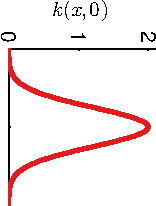
\includegraphics[width=\fwh,height=\fwb]{../figures/structure_examples/se_kernel}} &  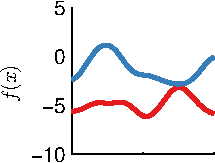
\includegraphics[width=\fwb,height=\fwh]{../figures/structure_examples/se_kernel_draws} & 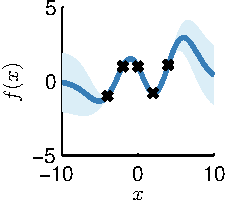
\includegraphics[width=\fwb,height=\fwh]{../figures/structure_examples/se_kernel_post} \\
squared-exp & \multicolumn{2}{c}{locally smooth} \\ \midrule
\rotatebox{90}{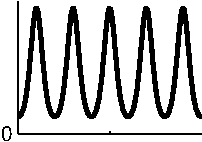
\includegraphics[width=\fwh,height=\fwb]{../figures/structure_examples/per_kernel}} &  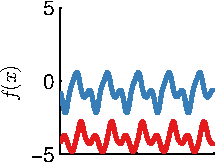
\includegraphics[width=\fwb,height=\fwh]{../figures/structure_examples/per_kernel_draws} & 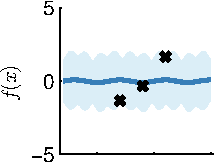
\includegraphics[width=\fwb,height=\fwh]{../figures/structure_examples/per_kernel_post} \\
periodic & \multicolumn{2}{c}{repeated structure} \\ \midrule
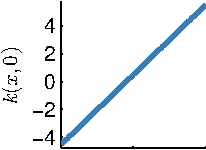
\includegraphics[width=\fwb,height=\fwh]{../figures/structure_examples/lin_kernel} &  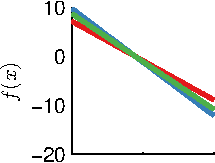
\includegraphics[width=\fwb,height=\fwh]{../figures/structure_examples/lin_kernel_draws} & 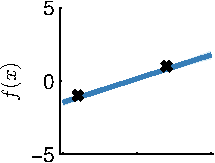
\includegraphics[width=\fwb,height=\fwh]{../figures/structure_examples/lin_kernel_post} \\
linear & \multicolumn{2}{c}{linear functions} \\ \midrule
\rotatebox{90}{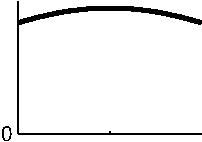
\includegraphics[width=\fwh,height=\fwb]{../figures/structure_examples/longse_kernel}} &  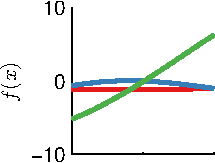
\includegraphics[width=\fwb,height=\fwh]{../figures/structure_examples/longse_kernel_draws} & 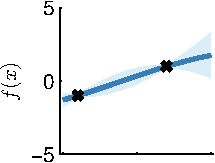
\includegraphics[width=\fwb,height=\fwh]{../figures/structure_examples/longse_kernel_post} \\
long-length SE & \multicolumn{2}{c}{slowly changing}
\end{tabular}
\caption{ Properties of basic kernels.  Left: base kernels. Centre:  draws from a \gp{} with that kernel.  Right: a GP posterior after conditioning on three datapoints.
\TBD{RBG: Do we need this figure?  It's pretty standard stuff, and it's largely subsumed by Figure 2.}}
\label{fig:basic_kernels}
\end{figure}

\newcommand{\fw}{2.6cm}
\begin{figure*}
\centering
\begin{tabular}{ccccc|c|c}
& & & & 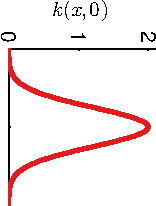
\includegraphics[width=\fw]{../figures/structure_examples/se_kernel} &  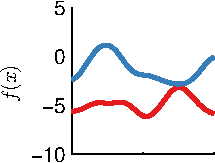
\includegraphics[width=\fw]{../figures/structure_examples/se_kernel_draws} & 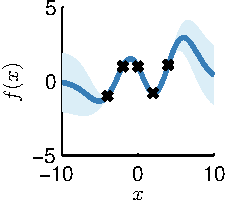
\includegraphics[width=\fw]{../figures/structure_examples/se_kernel_post} \\
& & & & 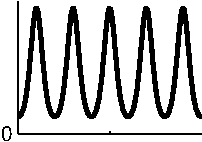
\includegraphics[width=\fw]{../figures/structure_examples/per_kernel} &  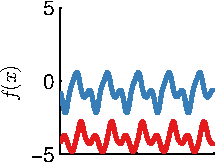
\includegraphics[width=\fw]{../figures/structure_examples/per_kernel_draws} & 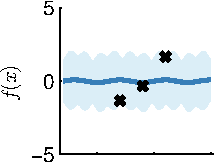
\includegraphics[width=\fw]{../figures/structure_examples/per_kernel_post} \\
& & & & 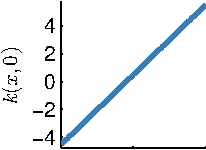
\includegraphics[width=\fw]{../figures/structure_examples/lin_kernel} &  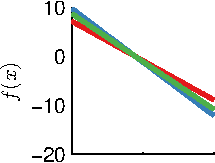
\includegraphics[width=\fw]{../figures/structure_examples/lin_kernel_draws} & 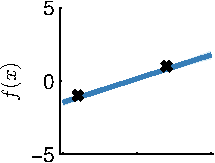
\includegraphics[width=\fw]{../figures/structure_examples/lin_kernel_post} \\
 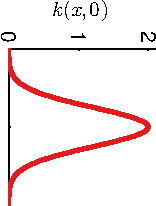
\includegraphics[width=\fw]{../figures/structure_examples/se_kernel} & $\times$ & 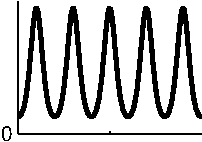
\includegraphics[width=\fw]{../figures/structure_examples/per_kernel} & = & 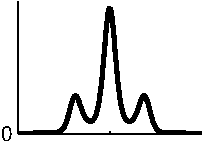
\includegraphics[width=\fw]{../figures/structure_examples/se_times_per} & 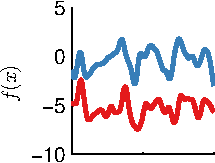
\includegraphics[width=\fw]{../figures/structure_examples/se_times_per_draws} & 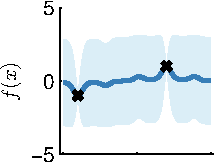
\includegraphics[width=\fw]{../figures/structure_examples/se_times_per_post} \\
  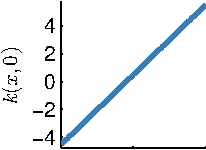
\includegraphics[width=\fw]{../figures/structure_examples/lin_kernel} & $\times$ & 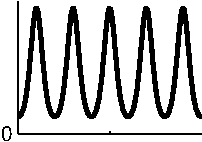
\includegraphics[width=\fw]{../figures/structure_examples/per_kernel} & = & 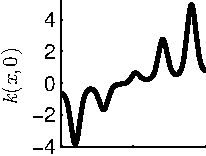
\includegraphics[width=\fw]{../figures/structure_examples/lin_times_per} & 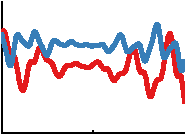
\includegraphics[width=\fw]{../figures/structure_examples/lin_times_per_draws} & 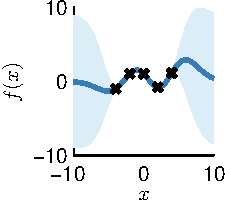
\includegraphics[width=\fw]{../figures/structure_examples/se_times_lin_post} \\
   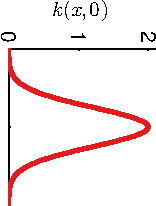
\includegraphics[width=\fw]{../figures/structure_examples/se_kernel} & $+$ & 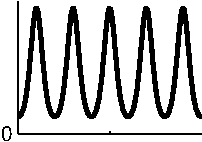
\includegraphics[width=\fw]{../figures/structure_examples/per_kernel} & = & 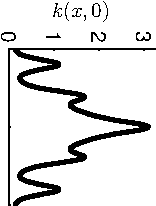
\includegraphics[width=\fw]{../figures/structure_examples/se_plus_per} & 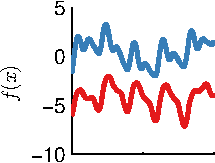
\includegraphics[width=\fw]{../figures/structure_examples/se_plus_per_draws} & 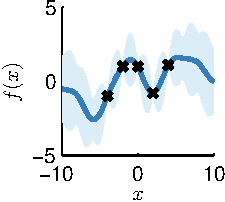
\includegraphics[width=\fw]{../figures/structure_examples/se_plus_per_post} \\
  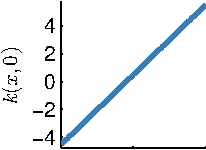
\includegraphics[width=\fw]{../figures/structure_examples/lin_kernel} & $+$ & 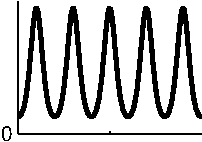
\includegraphics[width=\fw]{../figures/structure_examples/per_kernel} & = & 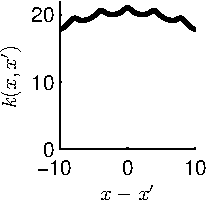
\includegraphics[width=\fw]{../figures/structure_examples/lin_plus_per} & 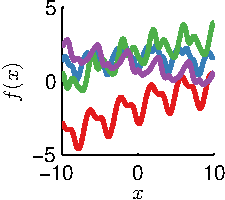
\includegraphics[width=\fw]{../figures/structure_examples/lin_plus_per_draws} & 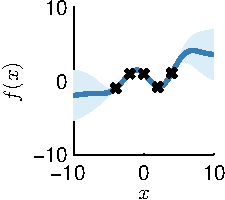
\includegraphics[width=\fw]{../figures/structure_examples/se_plus_lin_post} \\
   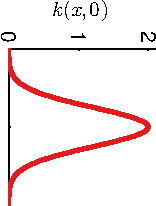
\includegraphics[width=\fw]{../figures/structure_examples/se_kernel} & $+$ & 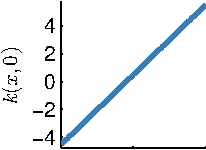
\includegraphics[width=\fw]{../figures/structure_examples/lin_kernel} & = & 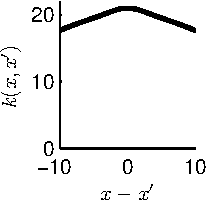
\includegraphics[width=\fw]{../figures/structure_examples/se_plus_lin} & 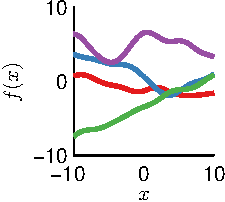
\includegraphics[width=\fw]{../figures/structure_examples/se_plus_lin_draws} & 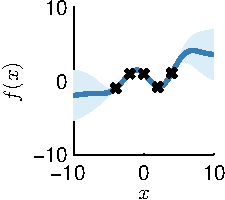
\includegraphics[width=\fw]{../figures/structure_examples/se_plus_lin_post} \\
   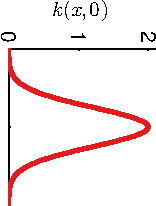
\includegraphics[width=\fw]{../figures/structure_examples/se_kernel} & $\times$ & 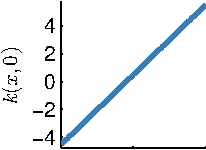
\includegraphics[width=\fw]{../figures/structure_examples/lin_kernel} & = & 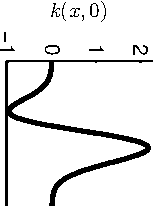
\includegraphics[width=\fw]{../figures/structure_examples/se_times_lin} & 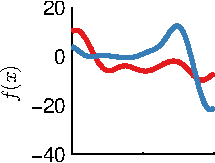
\includegraphics[width=\fw]{../figures/structure_examples/se_times_lin_draws} & \includegraphics[width=\fw]{../figures/structure_examples/se_times_lin_post} \\
base kernel & & base kernel & & combined kernel & draws from GP & GP posterior
\end{tabular}
\caption{ A draw from a sum of kernels corresponds to a sum of draws from the base kernels.  A draw from a product kernel prior has weaker long-range dependencies, and less long-range structure.
}
\label{fig:kernels}
\end{figure*}

\paragraph{Summation}

Summation of kernels corresponds to the summation of independent functions in the following sense.
Suppose ${\function_1 \dist \GP(0, \kernel_1)}$, and ${\function_2 \dist \GP(0, \kernel_2)}$ and are independent.
Then ${\function := \function_1 + \function_2 \dist \GP(0, \kernel_1 + \kernel_2)}$\footnotemark.
\footnotetext{Additionally, the posterior of the component functions conditioned on observations of the sum are analytically tractable. We make use of this in section\TBD{ add reference} and give derivations in the supplementary material.}

In one dimension, summing kernels can capture structures including multiple scales of variation\TBD{ reference a picture} or the sum of heterogeneous function types\TBD{ reference \eg SE + PE picture}.
In higher dimensions, summing kernels can correspond to decompositions of the form
\begin{equation}
\function((\inputVar_1, \inputVar_2)) = \function_1(\inputVar_1) + \function_2(\inputVar_2)
\end{equation}
\ie `independent' variation in different dimensions\TBD{ reference a plot}.

\paragraph{Multiplication}

Multiplication of kernels does not correspond to a simple decomposition of functions, but allows for the construction of different structures and is best understood on a case by case basis\fTBD{Better language?}.

For example, multiplying base kernels of the same form that act upon different dimensions of $\InputSpace$ can create the multidimensional generalisations of these kernels; this is true of \eg SE and LN\TBD{ reference a picture}.

Multiplying kernels of the same form in one dimension is often redundant \eg for SE kernels this just produces SE kernels with different parameters.
\TBD{What is PE $\times$ PE?}
However, multiplying kernels of different forms can give rise to interesting structures.

Multiplying a kernel, $\kernel$, by SE allows the structures implied by $\kernel$ to vary smoothly according the lengthscale of the SE kernel\TBD{ reference a picture}.
Multiplying a kernel by LN results in the amplitude of structures implied by $\kernel$ growing or shrinking linearly\TBD{ reference a picture}.
\fTBD{Could perhaps perversely claim that multiplying by periodic results in wiggles being added to previous structure?}

\fTBD{Can we do more than just give examples}

In general, multiplying kernels can be thought of as an `AND' operation when viewing kernels as a measure of similarity.
This arises since two points, $\inputVar,\inputVar'$, can only be considered similar by a product kernel function (\ie $\kernel_\textrm{prod}(\inputVar,\inputVar')$ is relatively large) if the points are considered similar by each component kernel function.

%\section{Gaussian Processes Priors}

%Gaussian processes are a flexible and tractable prior over functions, useful for solving regression and classification tasks\cite{rasmussen38gaussian}.
%The kind of structure which can be captured by a GP model is mainly determined by its \emph{kernel}: the covariance function.
%One of the main difficulties in specifying a Gaussian process model is in choosing a kernel which can represent the structure present in the data.
%For small to medium-sized datasets, the kernel has a large impact on modeling efficacy.
%\TBD{Note: The above paragraph is plagarized from my additive GP paper. -David} 

%
%The technique of constructing composite kernels using sums and products of existing kernels is not new \cite{rasmussen38gaussian} [more cites, Phil Hennig's astronomy work?].  
%However, the main contribution of this paper is to automate the search over kernel structures.

\section{Searching over structures}

\paragraph{A grammar for kernels}

The discussion above demonstrates that rich structure can be captured with summation and multiplication of simple base kernels.
We therefore consider searching over all kernel structures that can be expressed as sums and products of base kernels.

Formally\fTBD{Maybe Roger is well placed to write this?}, we start with a collection of base kernels applied to each input dimension individually; $\kernel_i$ denotes a kernel applied to input dimension $i$.
We denote sums and products of kernels as $\SumKernel(\expression,\ldots)$ and $\ProductKernel(\expression,\ldots)$ where $\expression$ represents an arbitrary kernel expression.
We then generate new expressions by repeatedly applying the following production rules to base kernels, sum kernels and product kernel within an expression.
\begin{center}
\begin{tabular}{rccc}
\textrm{Replacement} & $\kernel_i$ & $\to$ & $\kernel'_i$\\% & $\forall\, \kernel' $\\
\textrm{Addition} & $\kernel_i$ & $\to$ & $\kernel_i + \kernel'_j$\\% & $\forall\, j,\kernel' $\\
& $\SumKernel(e,\ldots)$ & $\to$ & $\SumKernel(e,\ldots,\kernel'_j)$\\% & $\forall\, j,\kernel' $\\
& $\ProductKernel(e,\ldots)$ & $\to$ & $\SumKernel(\ProductKernel(e,\ldots),\kernel'_j)$\\% & $\forall\, j,\kernel' $\\
\textrm{Multiplication} & $\kernel_i$ &  $\to$ & $\kernel_i \times \kernel'_j$\\% & $\forall\, j,\kernel'$\\
& $\SumKernel(e,\ldots)$ & $\to$ & $\ProductKernel(\SumKernel(e,\ldots),\kernel'_j)$\\% & $\forall\, j,\kernel' $\\
& $\ProductKernel(e,\ldots)$ & $\to$ & $\ProductKernel(e,\ldots,\kernel'_j)$\\% & $\forall\, j,\kernel' $\\
\end{tabular}
\end{center}
For example, applying the multiplication production rule to the sum in the expression $\SumKernel(\kernel_\textrm{SE},\kernel_\textrm{SE})$ could result in the new expression $\ProductKernel(\SumKernel(\kernel_\textrm{SE},\kernel_\textrm{SE}),\kernel_\textrm{PE})$ \ie a kernel representing a smooth function with two characteristic scales of variation is transformed into a kernel representing a locally periodic function with two scales of variation.

\paragraph{Remark on notation} The $\SumKernel,\ProductKernel$ notation is useful algorithmically and to describe the production rules but elsewhere we will use more conventional algebraic notation \ie the two kernels above would be written as $\kernel_\textrm{SE} + \kernel_\textrm{SE}$ and ${(\kernel_\textrm{SE} + \kernel_\textrm{SE}) \times \kernel_\textrm{PE}}$.

\paragraph{A greedy search algorithm}
The base kernels and production rules generate a tree structure over kernel expressions and we follow a greedy search to traverse this tree.
This requires a method of scoring a kernel expression, which we achieve by using the Bayesian Information Criterion (BIC)\TBD{ cite me} as an estimate of the marginal likelihood of some data given the kernel expression\footnotemark.
\footnotetext{We also experimented with using a Laplace approximation to the marginal likelihood\TBD{ cite} but this was found to be less numerically stable and could not be computed if an optimiser failed to find a true optimum.}
Specifically, we optimise the marginal likelihood of the data given specific kernel parameters\TBD{ using LBFGS - cite?}, randomly restarting previously unoptimised kernel parameters.
This is then adjusted by the number of parameters optimised\footnotemark to compute the BIC\fTBD{formula?}.
\footnotetext{Adjustments were made for obvious parameter redundancy \eg multiplicative terms in products of kernels.}

The search then proceeds by scoring all base kernels applied to all input dimensions.
The highest scoring kernel is then expanded by applying all production rules, and these kernel expressions are scored.
The production rules are then applied to the highest scoring kernel expression and the search continues iteratively until some fixed depth.

\paragraph{Example expressions}

\TBD{Draw a picture to show what our model includes \ie polynomial regression, nonparametric Fourier decomposition, GAM, additive kernels.}

\section{Related Work}

The technique of constructing composite kernels using sums and products of existing kernels is not new\fTBD{weak language}, and was demonstrated in detail in Chapter 5 of \cite{rasmussen38gaussian}, where the resulting posterior mean was also decomposed into a sum of component-wise means, although the posterior variance was not\fTBD{worth highlighting?}.

Compositional Model search for unsupervised learning: \cite{grosse2012exploiting}

Hyperkernels \cite{ong2002hyperkernels}

\paragraph{ANOVA Kernels}

Support vector regression with ANOVA decomposition kernels \cite{stitson1999support}

%\subsubsection{Smoothing spline ANOVA models}
A closely related procedure from the statistics literature is smoothing-splines ANOVA (SS-ANOVA)\cite{wahba1990spline, gu2002smoothing}.
An SS-ANOVA model is estimated as a weighted sum of splines along each dimension, plus a sum of splines over all pairs of dimensions, all triplets, etc, with each individual interaction term having a separate weighting parameter.
Because the number of terms to consider grows exponentially in the order, in practice, only terms of first and second order are usually considered.
Learning in SS-ANOVA is usually done via penalized-maximum likelihood with a fixed sparsity hyperparameter.
\TBD{We need to discuss how our model relates to this one - it's very similar!}

\paragraph{Hierarchical Kernel Learning}

In "High-Dimensional Non-Linear Variable Selection through Hierarchical Kernel Learning", Bach\cite{DBLP:journals/corr/abs-0909-0844} uses a regularized optimization framework to learn a weighted sum over an exponential number of kernels which can be computed in polynomial time.
The subsets of kernels considered by this method are restricted to be a \textit{hull} of kernels.\footnote{In the setting we are considering in this paper, a hull can be defined as a subset of all terms such that if term $\prod_{j \in J} k_j(\bf x, x')$ is included in the subset, then so are all terms $\prod_{j \in J / i} k_j(\bf x, x')$, for all $i \in J$.
For details, see \cite{DBLP:journals/corr/abs-0909-0844}.}
%Given each dimension's kernel, and a pre-defined weighting over all terms, HKL performs model selection by searching over hulls of interaction terms.
% \subsubsection{All-subsets kernel with uniform weightings}
%In \cite{DBLP:journals/corr/abs-0909-0844}, Bach also fixes the relative weighting between orders of interaction with a single term $\alpha$, computing the sum over all orders by:
%\begin{equation}
%\label{eqn:uniform}
%k_{a}({\bf x, x'}) = v_D^2 \prod_{d=1}^D \left(1 + \alpha k_{d}(x_{d}, x_{d}') \right)
%\end{equation}
%which has computational complexity $O(D)$.
%However, this formulation forces the weight of all $n$th order terms to be weighted by $\alpha^n$.

The main difficulty with the approach of \cite{DBLP:journals/corr/abs-0909-0844} is that hyperparameters are hard to set other than by cross-validation. 
%In contrast, our method optimizes the hyperparameters of each dimension's base kernel, as well as the relative weighting of each order of interaction. 

Accuracy versus interpretability in flexible modeling: Implementing a tradeoff using Gaussian process models \cite{plate1999accuracy}

%A related functional ANOVA GP model\cite{kaufman2010bayesian} decomposes the \emph{mean} function into a weighted sum of GPs.
%However, the effect of a particular degree of interaction cannot be quantified by that approach.
%Also, computationally, the Gibbs sampling approach used in \cite{kaufman2010bayesian} is disadvantageous.

\paragraph{Genetic Searches}

Evolving kernel functions for SVMs by genetic programming: \cite{diosan2007evolving}

A Genetic Programming based kernel construction and optimization method for Relevance Vector Machines: \cite{bing2010gp}

\paragraph{Equation Learning}

Equation discovery with ecological applications \cite{dzeroski1999equation}

Discovering admissible model equations from observed data based on scale-types and identity constraints \cite{washio1999discovering}

\paragraph{Multiple Kernel Learning}

\cite{christoudias2009bayesian} previously showed how mixtures of kernels can be learnt by gradient descent in the Gaussian process framework.
They call this \emph{Bayesian localized multiple kernel learning}.

\paragraph{Using DBNs to learn a kernel function}

\TBD{Cite relevant work by Salkhutdinov and Hinton}

\section{Decomposition}

\fTBD{This is a key part of the paper, so I think we should devote an entire section}

We demonstrate the decompositions produced by our method on two time series.
For the search we used $k = 1$, $D = 8$ and the kernels in Table~\ref{tbl:kernel_descriptions}.
%These were chosen to minimally allow the discovery of smooth functions, smooth periodic functions, rough functions and linear structure.
% \TBD{these were chosen to minimally (without parameter degeneracy e.g.~RQ could approximate SE and LN) allow the discovery of smooth functions, smooth periodic functions, rough functions and linear structure}.

%% --- Automatically generated by latex.py ---
% Exported at 2013-01-28 17:50:37.602844
\begin{table}[h!]
\begin{center}
\begin{tabular}{l | l l l}
   & \rotatebox{0}{ Description }  & \rotatebox{0}{ Parameters }  \\ \hline
SE & Squared-exponential  & lengthscale  \\
RQ & Rational Quadratic  & lengthscale, alpha  \\
LN & Linear  & none  \\
P & Piecewise Polynomial 1  & lengthscale  \\
MT & Mat\'{e}rn  & lengthscale  \\
\end{tabular}
\end{center}
\label{tbl:kernel_descriptions}
\end{table}


The sorts of structure implied by complex kernel might not be immediately interpretable.
However, there is one property of GPs that allows us to break down the signal into interpretable parts.
Specifically, a function $f \sim GP(0, k_1(x, x') + k_2(x,x')$, whose kernel is a sum of kernels, has the same distribution as a sum of two functions $\vf = \vf_1 + \vf_2$ where $\vf_1 \sim \gp( \vmu_1, k_1)$ and $\vf_2 \sim \gp( \vmu_2, k_2)$.
In addition, the posterior distributions over individual components after conditioning on data are also analytically tractable.

\fTBD{Move all maths to supplementary?}
The conditional distribution of a Gaussian $\vf_1$ conditioned on its sum with another Gaussian $\vf = \vf_1 + \vf_2$ where $\vf_1 \sim \gp( \vmu_1, k_1)$ and $\vf_2 \sim \gp( \vmu_2, k_2)$ is given by
\begin{align}
\vf_1^\star | \vf \sim \mathcal{N} \big( & \vmu_1^\star + \vk_1^\star (\vK_1 + \vK_2)\inv \left( \vf - \vmu_1 - \vmu_2 \right), \nonumber \\
& \vk_1^{\star\star} - \vk_1^\star (\vK_1 + \vK_2)\inv \vk_1^\star \big).
\end{align}
and the covariance between the two components, conditioned on their sum is given by:
\begin{align}
\cov(\vf_1^\star, \vf_2^\star) | \vf = \vk_1^{\star\tra} (\vK_1 + \vK_2)\inv \vk_2^\star
\end{align}
Derivations can be found in the supplementary material.
\fTBD{We can drop the star notation without losing much}

%These distributions express the posterior model uncertainty about different components of the signal, integrating over the possible configurations of the other components.
These expressions allow us to decompose the posterior into a sum of interpretable parts, and examine each one in turn.

\paragraph{Mauna Loa Atmospheric Carbon Dioxide}

As an example of a GP modeling problem where choosing an appropriate structure is critical, we revisit a dataset explored in \cite{rasmussen38gaussian}, pages 120-126, where a kernel was hand-tailored to fit a GP model to the dataset.

Figures \ref{fig:mauna_grow} show the posterior's increasingly appropriate model as the search depth increases on the Mauna Loa dataset.
Note in particular that, while the data can be smoothly interpolated a single base kernel model, the extrapolations improve dramatically as the search depth increases.

Figure \ref{fig:mauna_decomp} shows the complete posterior of the maximum depth $\gp$ regression model together with the additive components of the posterior.
The plot shows a very plausible extrapolation and highly interpretable components i.e.~a long-term trend, annual periodicity, medium-term deviations and short-term serially correlated `noise'.

\begin{figure}[h!]
\centering
\newcommand{\wmg}{8cm}  % width maunu growth
\newcommand{\hmg}{4cm}  % height maunu growth
\begin{tabular}{c}
 \includegraphics[width=\wmg,height=\hmg]{../figures/decomposition/03-mauna2003_max_level_0/03-mauna2003_all} \\ 
 \includegraphics[width=\wmg,height=\hmg]{../figures/decomposition/03-mauna2003_max_level_1/03-mauna2003_all} \\
 \includegraphics[width=\wmg,height=\hmg]{../figures/decomposition/03-mauna2003_max_level_2/03-mauna2003_all}
\end{tabular}
\caption{Posterior mean and variance for different depths of kernel search.  In the first row, the function is only modeled as a locally smooth function, and the extrapolation is extemely poor.  In the second, a periodic component is added, and the extrapolation is better.  At depth 3, the kernel can capture most of the relevant structure, and is able to extrapolate reasonably. \TBD{RBG: (1) I think we somehow need to visualize the lengthscales, to make it obvious that the SE kernels really mean different things. (2) Why isn't SE + PE the correct answer?  In the second model, is the SE capturing part of the periodic component, forcing us to move to a locally periodic model?  (3) In general, in these figures, shouldn't we report the original form of the kernel rather than the expanded form?  It's not obvious how to get from 2 to 3 in one step.}}
\label{fig:mauna_grow}
\end{figure}

\begin{figure}[h!]
\newcommand{\wmgd}{8cm}  % width mauna growth decomp
\newcommand{\hmgd}{3cm}  % height mauna growth decomp
\begin{tabular}{c}
 \includegraphics[width=\wmgd,height=\hmgd]{../figures/decomposition/03-mauna2003_max_level_8/03-mauna2003_all} \\ = \\
 \includegraphics[width=\wmgd,height=\hmgd]{../figures/decomposition/03-mauna2003_max_level_8/03-mauna2003_3} \\ + \\
 \includegraphics[width=\wmgd,height=\hmgd]{../figures/decomposition/03-mauna2003_max_level_8/03-mauna2003_4_zoom} \\ + \\
 \includegraphics[width=\wmgd,height=\hmgd]{../figures/decomposition/03-mauna2003_max_level_8/03-mauna2003_1} \\ + \\
 \includegraphics[width=\wmgd,height=\hmgd]{../figures/decomposition/03-mauna2003_max_level_8/03-mauna2003_2} \\
\end{tabular}
\caption{First row: The posterior on the Mauna Loa dataset after a search of depth 8.  Subsequent rows: automatic decomposition of Mauna Loa data.  The signal has been automatically decomposed into long-term, yearly periodic, medium-term anomaly and short-term noise components, respectively.}
\end{figure}
\label{fig:mauna_decomp}

\paragraph{Airline passenger data}

Figures \ref{fig:airline_grow} and \ref{fig:airline_decomp} show the corresponding plots for the airline data set (\TBD{describe me!}).
\TBD{Make similar observations of good performance and perhaps draw attention to the selection of a linear kernel}.

\begin{figure}[h!]
\centering
\newcommand{\wag}{8cm}  % width airline growth
\newcommand{\hag}{4cm}  % height airline growth
\begin{tabular}{c}
 \includegraphics[width=\wag,height=\hag]{../figures/decomposition/01-airline-months_max_level_0/01-airline-months_all} \\ 
 \includegraphics[width=\wag,height=\hag]{../figures/decomposition/01-airline-months_max_level_1/01-airline-months_all} \\
 \includegraphics[width=\wag,height=\hag]{../figures/decomposition/01-airline-months_max_level_2/01-airline-months_all} \\
 \includegraphics[width=\wag,height=\hag]{../figures/decomposition/01-airline-months_max_level_3/01-airline-months_all}
\end{tabular}
\caption{Posterior mean and variance for different levels of kernel search on the airline dataset.}
\label{fig:airline_grow}
\end{figure}


\begin{figure}[h!]
\centering
\newcommand{\wagd}{8cm}  % width airline growth decomp
\newcommand{\hagd}{4cm}  % height airline growth decomp
\begin{tabular}{c}
 \includegraphics[width=\wagd,height=\hagd]{../figures/decomposition/01-airline-months_max_level_8/01-airline-months_all} \\ 
 = \\ 
 \includegraphics[width=\wagd,height=\hagd]{../figures/decomposition/01-airline-months_max_level_8/01-airline-months_1} \\
 + \\
 \includegraphics[width=\wagd,height=\hagd]{../figures/decomposition/01-airline-months_max_level_8/01-airline-months_2} \\
 + \\
 \includegraphics[width=\wagd,height=\hagd]{../figures/decomposition/01-airline-months_max_level_8/01-airline-months_3}
\end{tabular}
\caption{First row:  The airline dataset and posterior after a search of depth 8.  Rows 2-4: Additive decomposition of posterior into long-term smooth trend, yearly variation, and short-term noise.  Note that the variance of the noise grows over time, making this a heteroskedastic model.}
\label{fig:airline_decomp}
\end{figure}

To evaluate the effectiveness of our method we performed two types of experiments.
First, we examined the ability of our algorithm to discover useful structure in one-dimensional datasets.  Second, we examined the predictive performance of our model on multi-dimensional datasets.
% testing the ability of the algorithm to infer both an accurate regression function estimate and to produce an interpretable decomposition of a regression function.
%The accuracy experiments show that our method consistently matches or beats previous state of the art regression methods (\TBD{not yet statistically significantly within each experiment - more experiments currently running\ldots}).
%The decomposition experiments produce highly interpretable decompositions of time series data and highly plausible extrapolations; a particularly rare property of naively applied (linear) smoothers (\TBD{justify comment - e.g.~local linear is just linear, GP Sq-Exp nose dives towards the mean}).

\section{Numerical evaluation}
\fTBD{Bad title name}

\subsection{Multidimensional datasets}

\paragraph{Bach Synthetic Dataset}
In addition to standard UCI repository datasets, we generated a synthetic dataset following the same recipe as \cite{DBLP:journals/corr/abs-0909-0844}.
% From a covariance matrix drawn from a Wishart distribution with 1024 degrees of freedom, we select 8 variables.
%We then construct the non-linear function $f(X) = \sum_{i=1}^4 \sum_{j=1+1}^4 X_i X_j + \epsilon$, which sums all 2-way products of the first 4 variables, and adds Gaussian noise $\epsilon$.
This dataset is one which can be predicted well by a kernel which is a sum of two-way interactions over the first 4 variables, ignoring the extra 4 noisy copies.
%
This dataset was designed by \cite{DBLP:journals/corr/abs-0909-0844} to demonstrate the advantages of HKL over a \gp{} with a SE-ARD kernel. 

%If the dataset is large enough, HKL can construct a hull around only those subsets of cross terms that are optimal for predicting the output.
%GP-ARD, in contrast, can only learn to ignore the noisy copy variables, but cannot learn to ignore the higher-term interactions between the predictive variables.
%However, a GP with an additive kernel can learn both to ignore irrelevant variables, and to ignore certain orders of interaction.
%In this example, the additive GP is able to recover the relevant structure.

[TODO: Describe concrete, pumadyn, servo and housing]

\subsection{Details of Methods Used}

\paragraph{Linear regression} was included as a baseline. A likelihood score was obtained by setting the noise variance to the empirical variance on the training set.

\paragraph{Generalized Additive Models} are models for which the posterior mean can be expressed $\expect[f(\vx)] = \sum_{d=1}^D f_d(x_d)$.  
In our experiments, this model is implemented through a GP whose kernel is a sum of sq-exp kernels across dimensions.  
This model, denoted GP GAM, was included to demonstrate that the gain in predictive performance was not simply due to the inclusion of additive structure.

\paragraph{Hierarchical Kernel Learning}	
HKL\footnote{Code for HKL available at \texttt{http://www.di.ens.fr/\textasciitilde fbach/hkl/}} was run using the all-subsets kernel, which corresponds to the same set of kernels as considered by the additive GP with a squared-exp base kernel.

\paragraph{Additive Gaussian Processes} \cite{duvenaud2011additive11} is a Gaussian process model whose kernel imlicitly sums over all $2^D$ possible products of one-dimensional base kernels.  
However, this model's parameterization is not as flexible as the kernels expressible in our grammar.

\paragraph{Structure Search}
All of the experiments in this paper were performed using the standard GPML toolbox\footnote{Available at \texttt{http://www.gaussianprocess.org/gpml/code/}}; code to perform all experiments is available at the authors' website.\TBD{How true will this be?}


\subsection{Results}

%$k = 1$, $D = 8$, kernels are SE and RQ (\TBD{currently running other experiments that may be more canonical}).
%We have extended the comparison of \cite{duvenaud2011additive11} to include our method.
%5 data sets were split into 10 equally sized folds.
Datasets were evaluated on both mean-squared error and predictive likelihood on random 10-fold splits.
%For each fold of each data set we trained each method on the other 9 folds, and then computed predictive mean squared error (MSE) and mean negative predictive log likelihood on the held out fold (data missing at random \TBD{we could likely do much better by creating folds that remove continuous regions if extrapolation ability carries over to high dimensional data}.
Results are presented in tables \ref{tbl:Regression Mean Squared Error} and \ref{tbl:Regression Negative Log Likelihood}.
%
% --- Automatically generated by resultsToLatex2.m ---
% Exported at 28-Jan-2013 15:53:45
\begin{table*}[ht!]
\caption{{\small
Regression Mean Squared Error
}}
\label{tbl:Regression Mean Squared Error}
\begin{center}
\begin{tabular}{l | r r r r r}
Method & \rotatebox{0}{ bach  }  & \rotatebox{0}{ concrete  }  & \rotatebox{0}{ puma }  & \rotatebox{0}{ servo }  & \rotatebox{0}{ housing }  \\ \hline
Linear Regression & $1.031$ & $0.404$ & $0.641$ & $0.523$ & $0.289$ \\
GP GAM & $1.259$ & $0.149$ & $0.598$ & $0.281$ & $0.161$ \\
HKL & $\mathbf{0.199}$ & $0.147$ & $0.346$ & $0.199$ & $0.151$ \\
GP Squared-exp & $\mathbf{0.045}$ & $0.157$ & $0.317$ & $0.126$ & $\mathbf{0.092}$ \\
GP Additive & $\mathbf{0.045}$ & $\mathbf{0.089}$ & $\mathbf{0.316}$ & $\mathbf{0.110}$ & $0.102$ \\
%22-Jan & $\mathbf{0.513}$ & $\mathbf{0.089}$ & $\mathbf{0.312}$ & $\mathbf{0.095}$ & $\mathbf{0.091}$ \\
\hline
Structure Search & $\mathbf{0.044}$ & $\mathbf{0.087}$ & $\mathbf{0.315}$ & $\mathbf{0.102}$ & $\mathbf{0.082}$
\end{tabular}
\end{center}
\end{table*}
% End automatically generated LaTeX

% --- Automatically generated by resultsToLatex2.m ---
% Exported at 28-Jan-2013 15:53:45
\begin{table}[h!]
\caption{{\small
Regression Negative Log Likelihood
}}
\label{tbl:Regression Negative Log Likelihood}
\begin{center}
\begin{tabular}{l | r r r r r}
Method & \rotatebox{0}{ bach  }  & \rotatebox{0}{ concrete  }  & \rotatebox{0}{ puma }  & \rotatebox{0}{ servo }  & \rotatebox{0}{ housing }  \\ \hline
Linear Regression & $2.430$ & $1.403$ & $1.881$ & $1.678$ & $1.052$ \\
GP GAM & $1.708$ & $0.467$ & $1.195$ & $0.800$ & $0.457$ \\
GP Squared-exp & $\mathbf{-0.131}$ & $0.398$ & $0.843$ & $0.429$ & $0.207$ \\
GP Additive & $\mathbf{-0.131}$ & $\mathbf{0.114}$ & $\mathbf{0.841}$ & $\mathbf{0.309}$ & $0.194$ \\
22-Jan & $\mathbf{0.346}$ & $\mathbf{0.134}$ & $\mathbf{0.835}$ & $\mathbf{0.241}$ & $\mathbf{0.138}$ \\
28-Jan & $\mathbf{-0.141}$ & $\mathbf{0.065}$ & $\mathbf{0.840}$ & $\mathbf{0.265}$ & $\mathbf{0.059}$ \\
\end{tabular}
\end{center}
\end{table}
% End automatically generated LaTeX

%
Our method outperforms the other methods in all tests. 
%Some points for discussion
%\begin{itemize}
%\item Experiments just using SE kernel can outperform additive kernel surprisingly. This is presumably a regularisation effect of using a finite depth search and/or BIC. We could make this a more Bayesian result (i.e.~more a property of the model) by placing a prior on kernels that depends on the number of components.
%\item Need to discuss design choices e.g.~$k$, depth of search, base kernels.
%\end{itemize}

\section{Discussion}

Machine learning can be more data-driven, analogous to the high-thoughput approaches being used in biology. 

In this paper, we introduced an automated search over composite kernels, defining the search space through a simple grammar consisting of a set of one-dimensional base kernels and operations which combine those kernels.

We examined the composite kernels discovered by this search on several datasets, and demonstrate that they can recover known structure, and result in state-of-the-art predictive performance.  We further demonstrated an automated decomposition of the posterior into a sum of interpretable components.

%\section{Future Work}

%\TBD{RBG: Do we need this section?  Bill hates future work sections since they basically just give the reviewers a list of things to complain about.}

%\paragraph{Support Vector Machines} Structure search could be used to select kernels for support vector machines, using cross-validated prediction error as an objective function.

%However, it would be presumably quite difficult to learn the moderate number of kernel hyperparameters present in composite kernels using only cross-validation.

%\paragraph{Noise Models and Mean Functions}
%The models used in this paper all assumed Gaussian noise, as well a constant mean function for the Gaussian process.
%A more sophisticated approach might also define grammars over composite mean functions and noise models.
%However, in most cases, the covariance function can express structure that might be expressed in the mean function, and often in a more flexible way.
%The same can be said about noise models - for instance, a t-noise can be approximated by a sum of sq-exp kernels with very small lengthscales, but output variances which vary widely.


%\paragraph{Bayes model averaging}
%A natural extension of this work is to average over models in the grammar with a Bayes model averaging approach.
%This would mean augmenting our grammar with a prior over kernel structures, and approximately integrating over both structures and kernels.  

%In the first few levels of the search, where the difference between likelihoods of different kernel structures is usually high, model averaging might not make a substantial difference in terms of prediction.
%However, at deeper levels of the kernel search, integrating over structures and parameters would address overfitting concerns.

%\paragraph{Parsimony}
%Integrating over kernel structures raises the problem of reporting interpretable structures to the user.
%Currently, this is achieved through the use of the BIC complexity penalty, and reporting only the highest-scoring structure found.
%In experiments which used the more sophisticated Laplace approximation as a complexity penalty, the kernels found were more complicated.

%\paragraph{Bayesian Optimization} 
%The greedy search strategy used in this paper is rudimentary.  A natural extension of this work would be a model-based search over composite kernels, where the results of previous searches are used to propose informative directions.  This would be an example of ``meta-learning''.
%\cite{snoek2012practical} [also cite Lizotte, de Frietas]
%
%\paragraph{A Kernel between kernels}
%Placing a \gp{} model on the log-likelihood of different kernels would require constructing a kernel on kernels, as in \cite{ong2002hyperkernels}.

\subsubsection*{Acknowledgements}

\bibliographystyle{format/icml2013}
\bibliography{gpss}
\end{document}
